%!TEX root = ../rapport.tex
%!TEX encoding = UTF-8 Unicode

% Chapitres "Introduction"

% modifié par Francis Valois, Université Laval
% 31/01/2011 - version 1.0 - Création du document


\label{s:experimentation}
\chapter{Rapport}
\label{cha:projet}
Ce laboratoire vise premièrement à concevoir une boucle de régulation dans le domaine continu ainsi que la chaîne d'acquisition de données et implanter le système sous forme analogique et numérique.
\section{Préparation}
\begin{equation}
	G_p(s) = \frac{-12s + 1}{(22s +1)(5s+1)}
\end{equation}
On note premièrement la présence d'un zéro non inversible et de deux pôles stables de premier ordre. On choisit la constante de temps du pôle dominant comme constante de temps du régulateur PI, en effectuant l'approximation du système par un système de premier ordre sans retard. ($T_i = 22$). Il faut par la suite ajuster le gain du contrôleur en boucle fermée afin d'obtenir un dépassement maximal de 5\% pour un échelon de consigne. Pour ce faire, il est très laborieux de procéder par une méthode théorique (fixer $\omega_0$ comme une fonction de $K_C$ et déterminer la transformée inverse qui permet de satisfaire les exigences demandées). Il est préférable de procéder par itérations successives au moyen de l'utilitaire sisotool de Matlab. 
\paragraph{} On détermine premièrement la fonction de transfert en boucle ouverte (G)
\begin{equation}
G(s) = G_c(s) G_p(s) = 	\frac{-12s + 1}{(22s +1)(5s+1)} \times \frac{K_c (1 + 22s)}{22s} = \frac{K_c(-12s + 1)}{22s(5s + 1)}
\end{equation}
On détermine par la suite la fonction de transfert en boucle fermée (H)
\begin{equation}
H(s) = \frac{G(s)}{1 + G(s)} = \frac{K_c(-12s + 1)}{22s(5s+1) + K_c(-12s + 1)} = \frac{K_c(-12s + 1)}{110s^2 + (22 - 12K_c)s + K_c}
\end{equation} 
Au moyen de l'utilitaire sisotool de Matlab, on obtient un réglage optimal avec un gain $K_p = 0.748$. La méthode employée est une méthode par tâtonement, nous avons fixé la valeur de la constante de temps du régulateur et nous avons ajuster le gain de manière à respecter la spécification en dépassement en boucle fermée. L'utilitaire trace la réponse en boucle fermée et calcule la valeur du dépassement pour chacune des configurations. Il est possible de tracer la réponse en boucle fermée obtenue et de montrer le dépassement calculé de 4.85\%. Cela est réalisé à la figure \ref{fig1}
\begin{figure}[htbp]
\centering
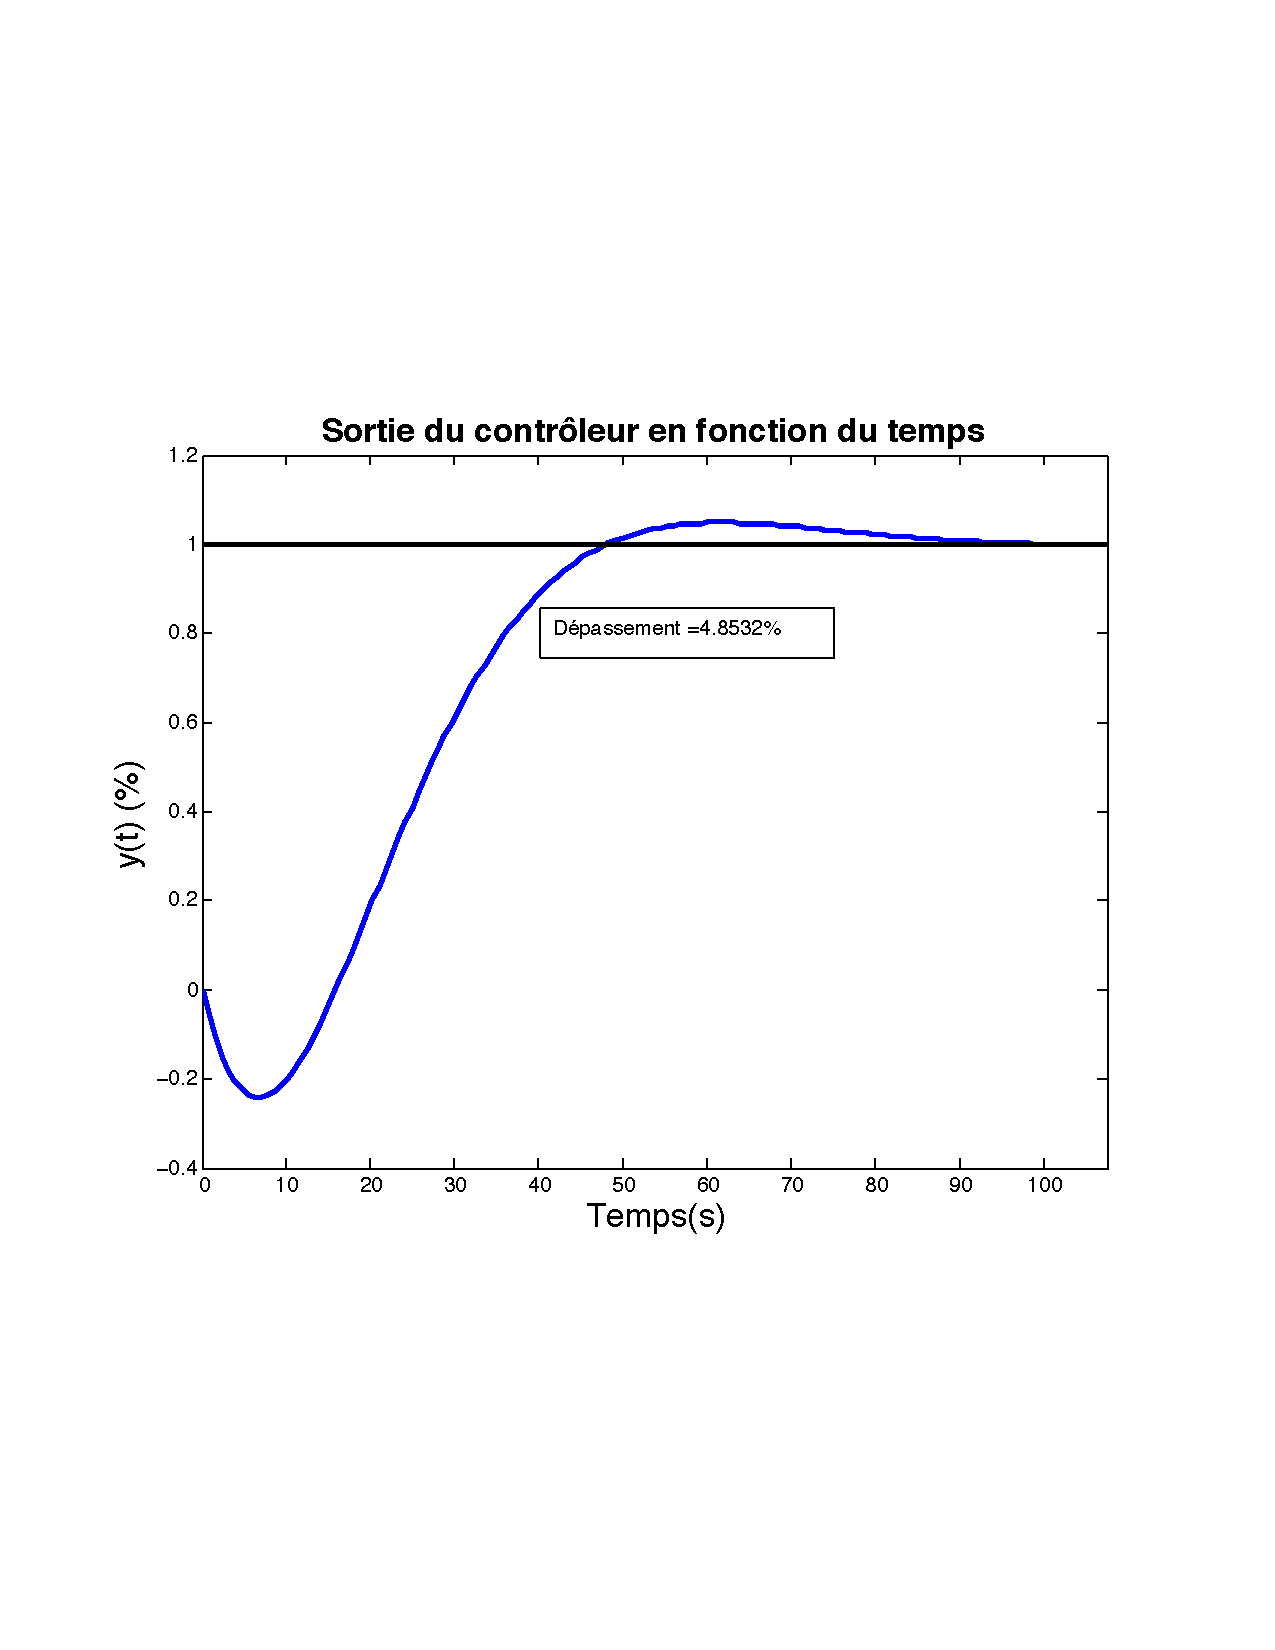
\includegraphics[scale=0.6]{figure_output_theorie.pdf}
\caption{Réponse temporelle désirée au moyen d'un réglage paramétrique effectué à l'aide de l'utilitaire sisotool}
\label{fig1}
\end{figure}
On a donc que la fonction de transfert du régulateur est la suivante:
\begin{equation}
G_c(s) = \frac{0.748(1 + 22s)}{22s}
\end{equation} 
Au moyen de Matlab et de l'utilitaire ltiviewer, on détermine que la bande passante du système en boucle fermée (3dB) est égale à 0.126rad. On peut observer l'allure de la fonction de transfert $G(s)$ à la figure \ref{fig2} On peut ensuite noter que la fonction en boucle ouverte  Il est par la suite possible de déterminer, à l'aide de la fonction margin, la marge de gain et la marge de phase ainsi que les fréquences auxquelles ces paramètres sont mesurés. La marge de gain ($M_g$) est égale à 7.79dB à une fréquence de 0.129 rad/s. La marge de phase ($M_p$) est égale à 56° à une fréquence de 0.0365 rad/s.
\paragraph{} On détermine par la suite que la fréquence d'échantillonnage devra être de $30\omega_b$, soit $\omega_s = 3.78 rad/s$. On détermine par la suite que pour obtenir une atténuation de 20dB à $\omega_s$ avec un premier ordre, il est nécessaire que la coupure du filtre soit exactement à une décade avant la fréquence $\omega_s$, on choisira donc une coupure à 0.378 rad/s. La fonction de transfert résultante du filtre sera la suivante:
\begin{equation}
G_f = \frac{1}{2.6455s +1}
\end{equation}
La constante de temps du filtre est obtenue en prenant l'inverse de la fréquence de coupure ($\frac{1}{0.378} = 2.6455$).La période d'échantillonnage est de $T = \frac{2 \pi}{3.78} =1.6622 s$. On approxime la fonction de transfert du bloqueur d'ordre 0 par $G_{BOZ}(s) = \times e^{-0.8311s}$. Le bloqueur d'ordre 0 réduit la marge de phase de 1.74 degrés, selon l'outil margin de matlab. Il est possible d'en visualiser l'impact sur la fonction de transfert de $G(s)$ à la figure \ref{fig3} La constante de temps de notre filtre anti-repliement ($T_f$) est égale à 2.6455 sec. L'atténuation du filtre à la fréquence $\omega_s$ est exactement de -20dB. L'atténuation du filtre à la fréquence $\omega_N$ est de -14.2dB. Le filtre anti-repliement apporte une réduction de marge de phase de 5.32 degrés. La marge de phase résultante du système est de 48.9 degrés. On peut voir l'impact du filtre anti-repliement sur la fonction de transfert en boucle ouverte à la figure \ref{fig4}
\begin{figure}... j
\centering
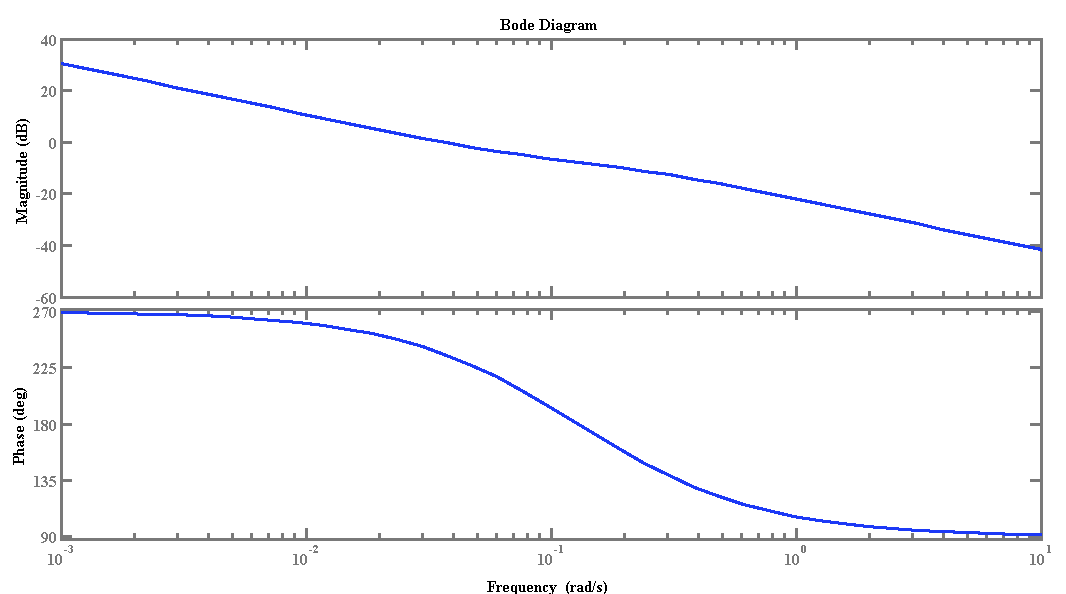
\includegraphics[scale=0.4]{G_s_base.png}
\caption{Réponse en fréquence du système en boucle ouverte (sans la présence de filtre anti-repliement ni de bloqueur d'ordre 0)}
\label{fig2}
\end{figure}
\begin{figure}
\centering
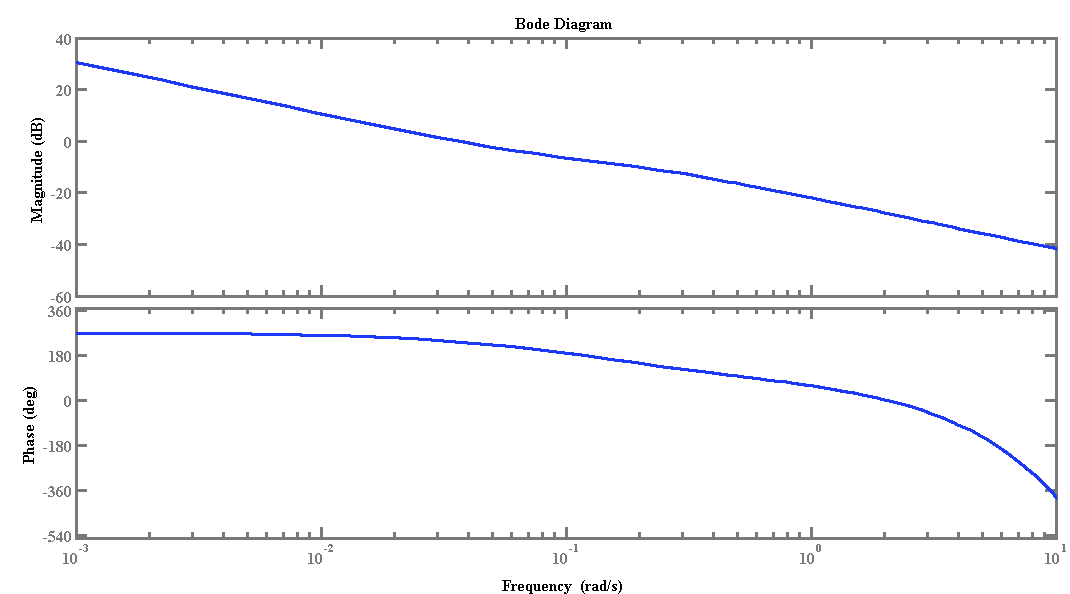
\includegraphics[scale=0.4]{G_s1.png}
\caption{Réponse en fréquence du système en boucle ouverte avec la présence du bloqueur d'ordre 0 (sans la présence de filtre anti-repliement)}
\label{fig3}
\end{figure}
\begin{figure}
\centering
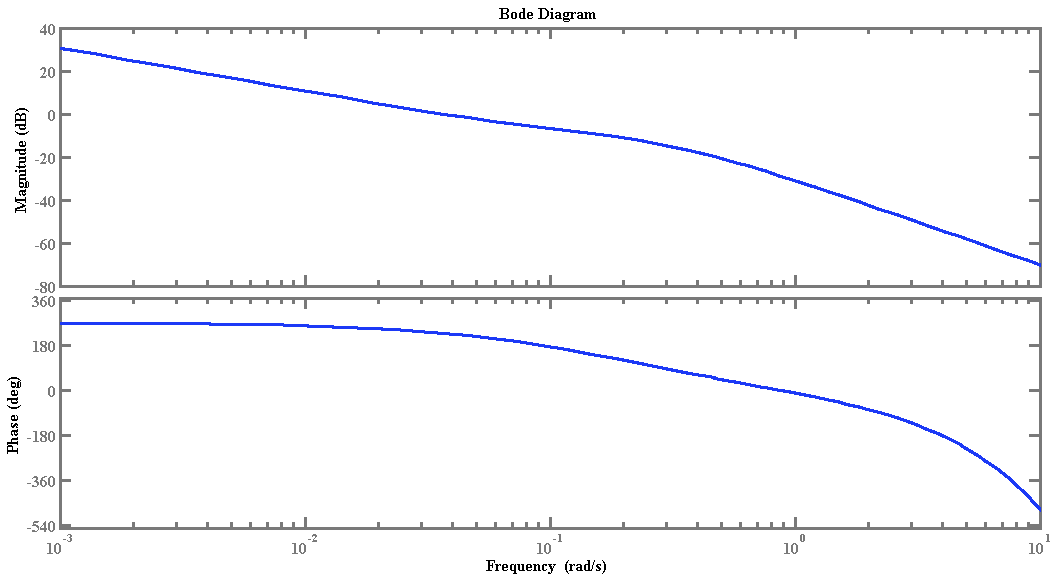
\includegraphics[scale=0.4]{G_s2.png}
\caption{Réponse en fréquence du système en boucle ouverte avec la présence du bloqueur d'ordre 0 et du filtre anti-repliement}
\label{fig4}
\end{figure}
\section{Expérimentation}
\subsection{Implantation du procédé analogique}
L'identification du procédé a été réalisée selon le schéma bloc présenté à la figure \ref{fig5}. La mise en parallèle des deux systèmes, l'ajustement du gain du second système et le changement de signe dans le premier système nous permet d'obtenir le zéro à la fréquence désirée au numérateur. 

\begin{figure}[htb]
\centering
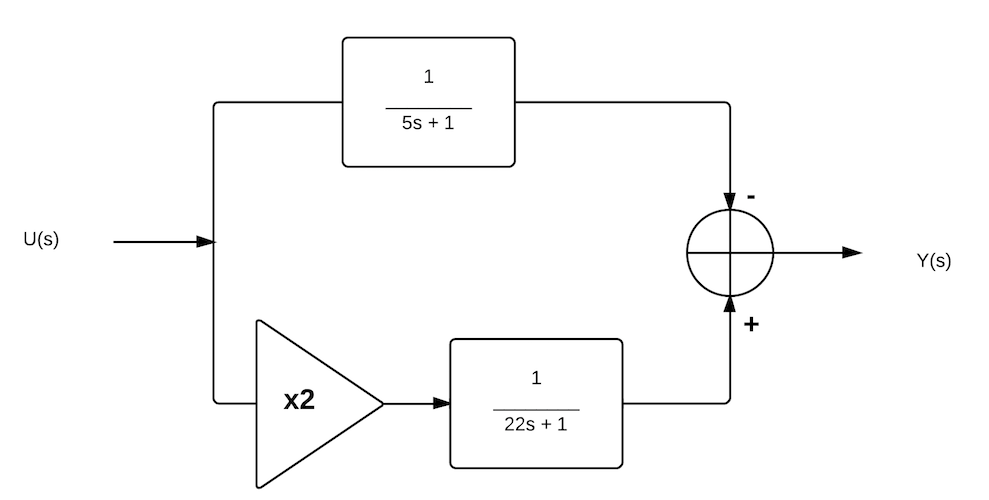
\includegraphics[scale=0.3]{Gp.png}
\caption{Schéma bloc du procédé tel qu'implanté au laboratoire}
\label{fig5}
\end{figure}
\begin{figure}[htb]
\centering
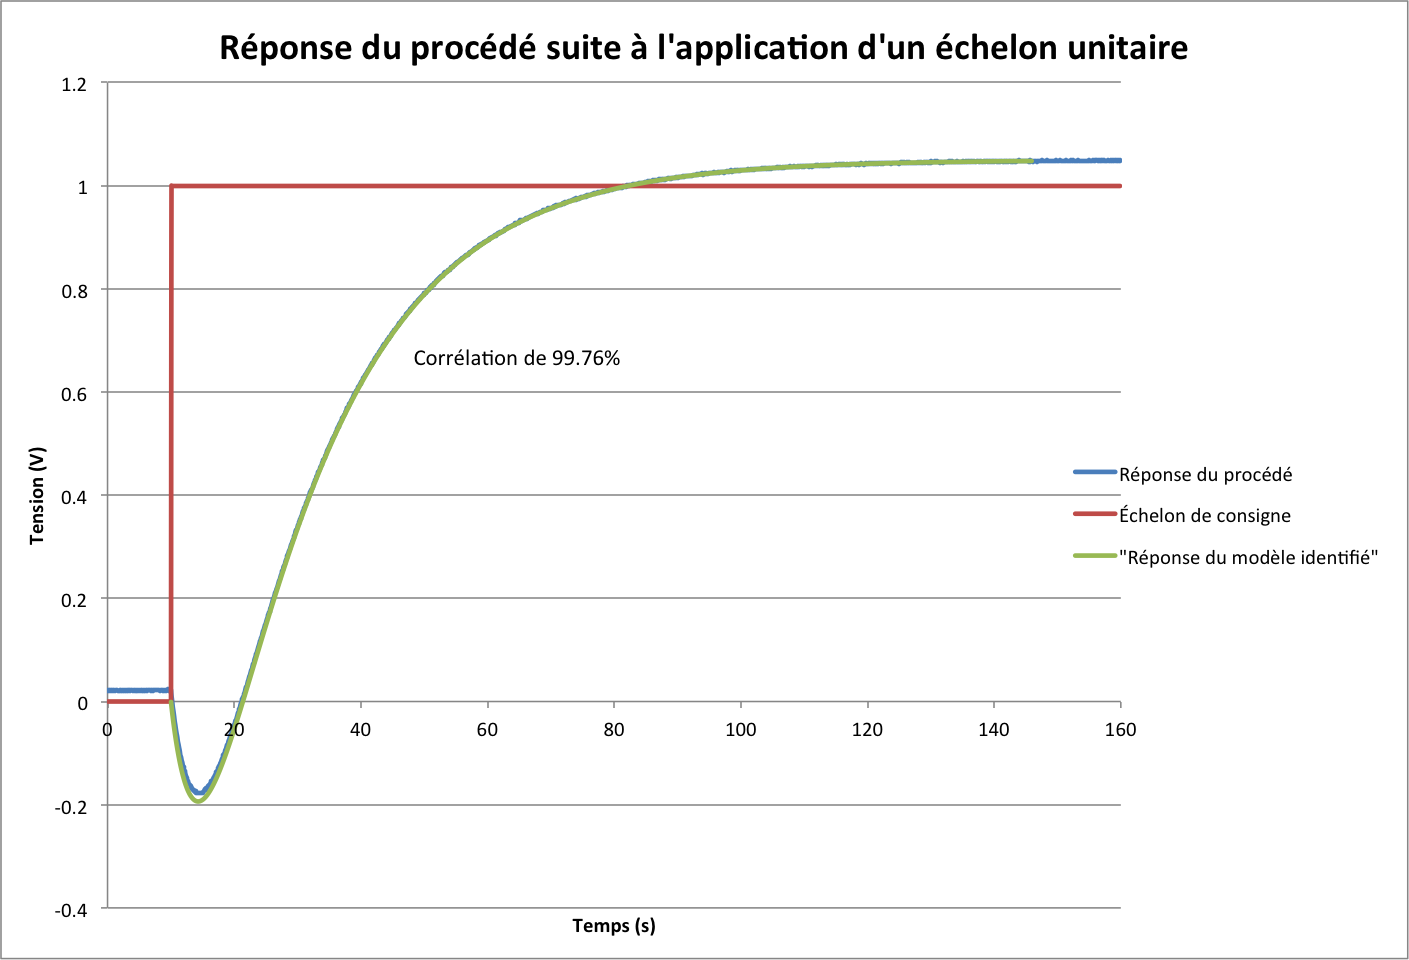
\includegraphics[scale=0.6]{fig_modele.png}
\caption{Comparaison de l'essai d'identification du procédé avec le modèle identifié}
\label{fig7}
\end{figure}
\subsection{Identification du procédé analogique}
\label{identification_procede_analogique}
Le système identifié expérimentalement au moyen de Ident possède un pôle dominant dont la constante de temps $T_1$ est égale à $19.4906$s La constante de temps du second pôle est égale à $x$s. La constante de temps du zéro est égale à $y$s et le gain de la fonction de transfert est égal à $z$. La corrélation indiquée par ident tourne autour de 99.7\%.La comparaison des essais d'identificaion du modèle théorique et pratique sont présentés à la figure \ref{fig7}. La fonction de transfert du procédé implanté est la suivante:
\begin{equation}
\label{eq1}
G_p = 1.0495 \times \frac{1-9.3097s}{(1+4.5829s)(1+19.4906s)}
\end{equation} 

\subsection{Conception du régulateur  analogique}
\begin{figure}[htb]
\centering
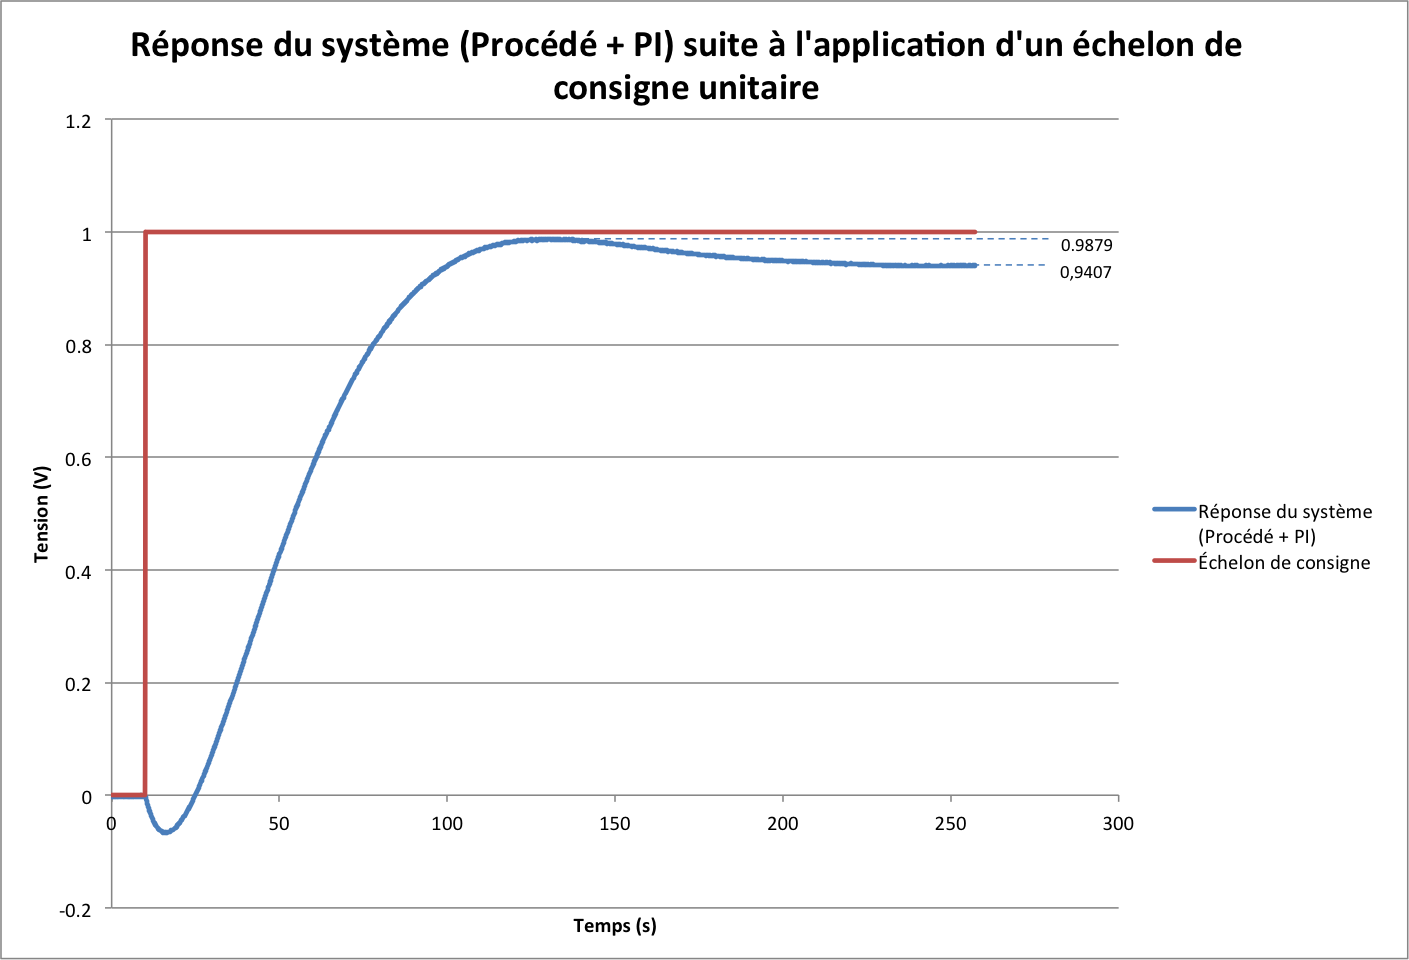
\includegraphics[scale=0.6]{fig_essai_analogique.png}
\caption{Essai de validation des performances du régulateur PID calculé au moyen de matlab}
\label{fig8}
\end{figure}\
\begin{figure}[htb]
\centering
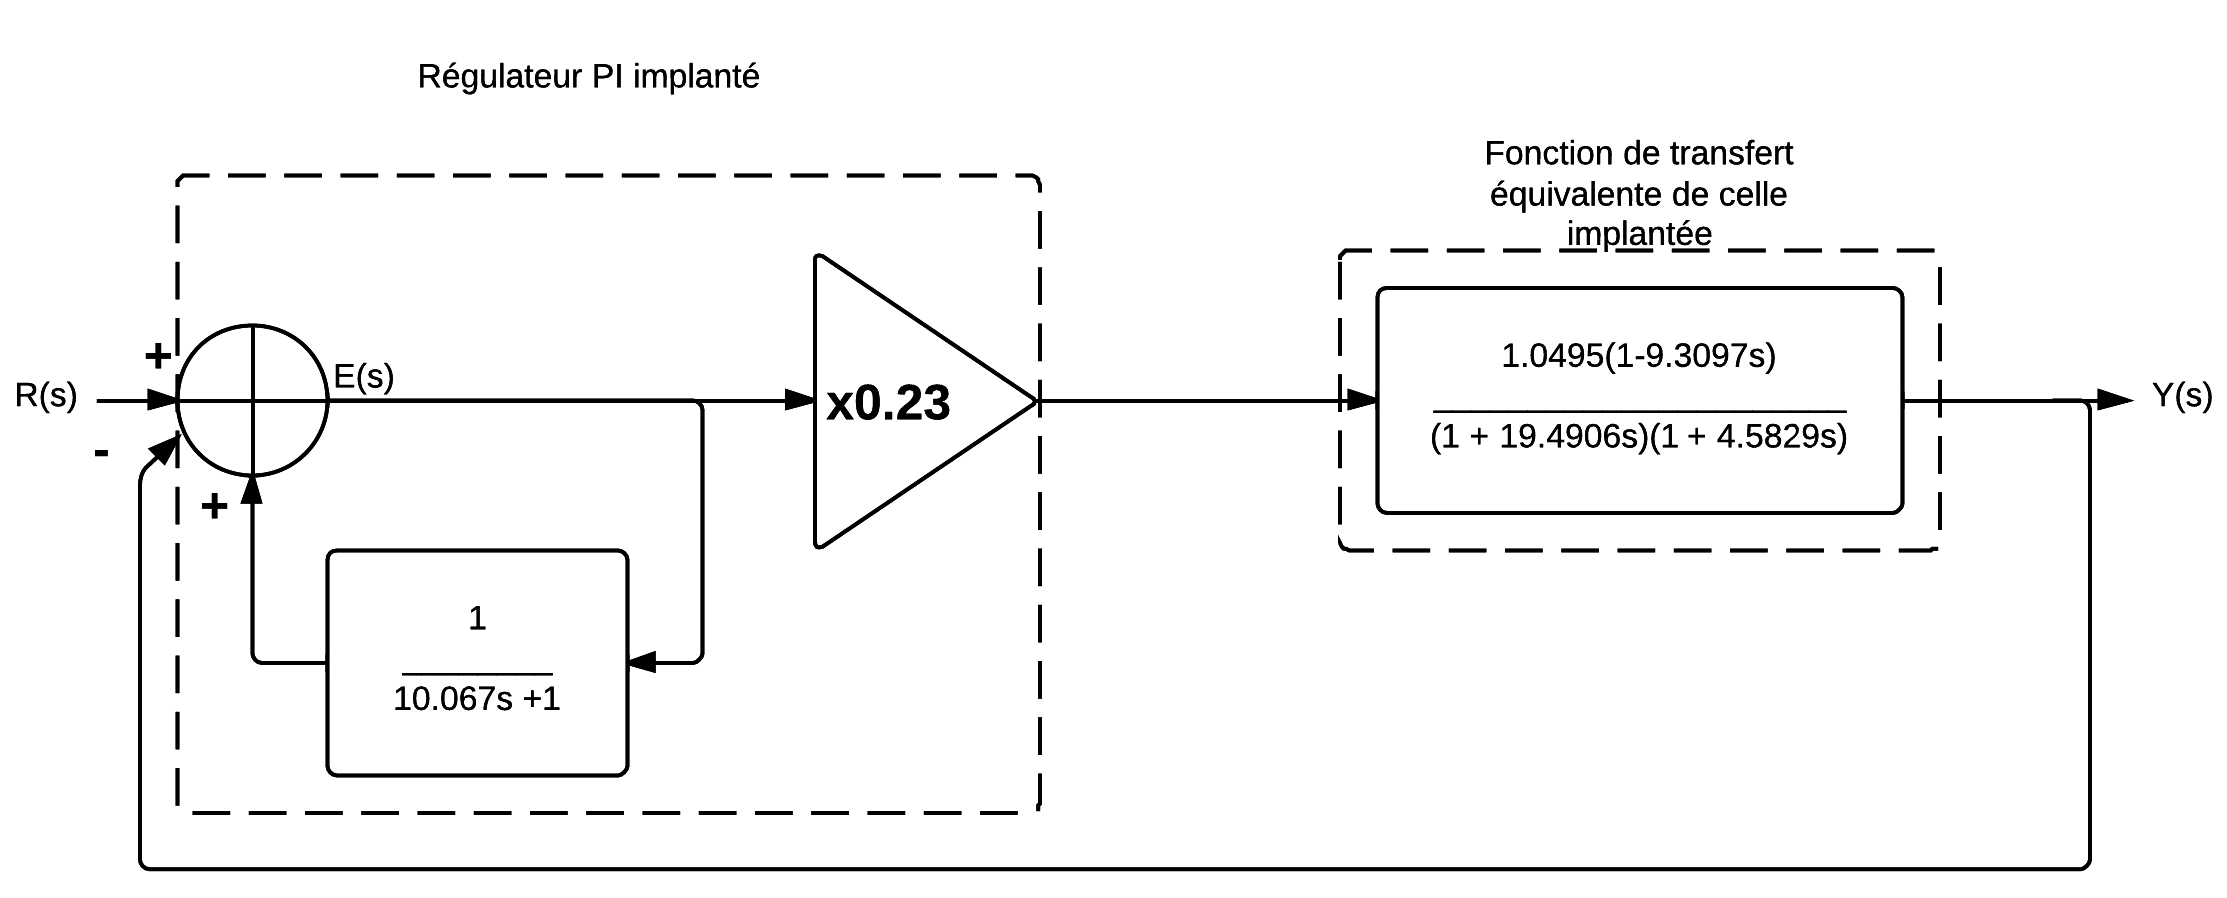
\includegraphics[scale=0.2]{procede_regulateur_analogique.png}
\caption{Essai de validation des performances du régulateur PID calculé au moyen de matlab}
\label{fig9}
\end{figure}
Le schéma bloc du régulateur analogique implanté est présenté à la figure \ref{fig9}. Les données réelles (identifiées) du procédé et du régulateur ont été employées pour rendre le schéma plus juste. Le zéro variable de notre montage ne nous permet pas d'atteindre une constante de temps supérieure à $10.067$s (le potentiomètre atteignant la limite supérieure de sa plage). Les calculs sont effectués avec une constante de temps du régulateur étant égale à $10.067$s. Tout comme dans la méthode exploitée dans la préparation de laboratoire, nous utilisons cette constante de temps et nous traçons la réponse en boucle ouverte. Nous limitons par la suite le dépassement à 5\% au moyen du gain du régulateur. Le gain déterminé à l'aide de l'outil sisotool est de 0.23. La réponse obtenue au moyen du régulateur analogique calibré avec sisotool est présentée à la figure \ref{fig8}. On remarque qu'il y a une erreur statique entre la réponse souhaitée et et la réponse en régime permanent, le dépassement est bel et bien de 5\%, tout comme cela avait été calculé.  La fonction de transfert du régulateur ($G_c(s)$) est présentée dans l'équation suivante:
\begin{equation}
G_c = \frac{0.23(1 + 10.067s)}{10.067s}
\end{equation}
\subsection{Conception du régulateur numérique}
\begin{figure}[htbp]
\centering
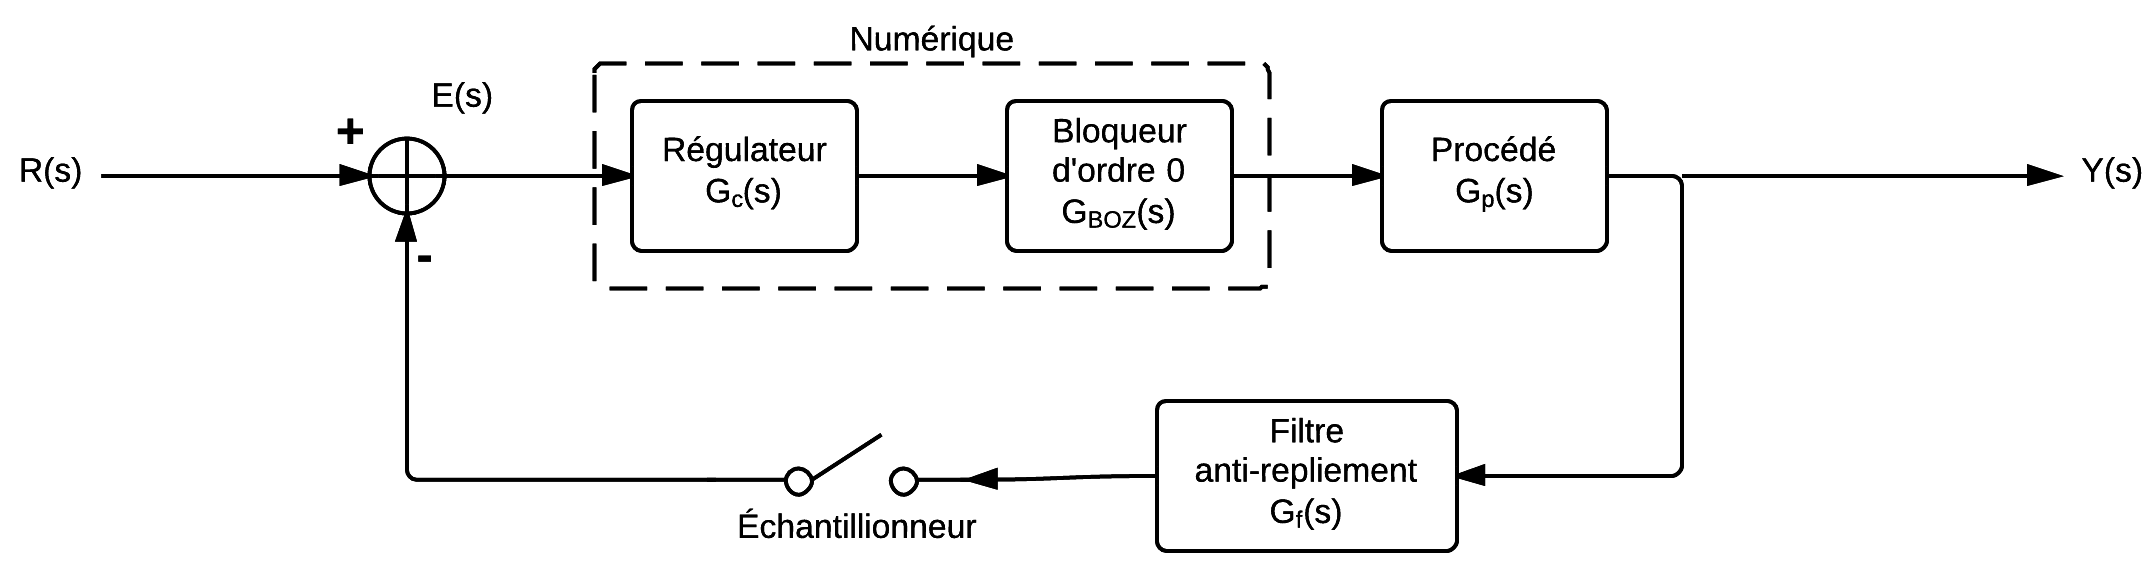
\includegraphics[scale=0.2]{Schema_numerique.png}
\caption{Schéma bloc du système avec asservissement numérique}
\label{fig7}
\end{figure}
Il est possible de visualiser l'implantation du régulateur numérique au moyen du schéma bloc présenté à la figure \ref{fig5}. On constate que l'implantation numérique suggère l'ajout d'un bloc de filtrage anti-repliement ainsi que d'un bloqueur d'ordre zéro (qui permet de maintenir la commande constante entre 2 échantillons.) La fonction de transfert du procédé est celle qui a été identifiée à la section \ref{identification_procede_analogique}. Sa fonction de transfert est celle présentée à l'équation \ref{eq1}. Lors des essais avec le régulateur numérique, nous avons dû ajusté le gain proportionnel de manière à respecter le critère de 5\% de dépassement maximal. L'utilisation d'un gain de 0.23 conduisait à une réponse beaucoup moins agressive et qui n'était pas comparable à la régulation analogique. Le gain ainsi ajusté est de 1.16. La fonction de transfert résultante du régulateur est présentée dans l'équation suivante:
\begin{equation}
G_c^{'} = \frac{1.16(1 + 10.067s)}{10.067s}
\end{equation}
\paragraph{}Le filtre anti-repliement a été implanté de manière analogique. La bande passante du signal (mesurée à l'aide de l'outil sisotool de matlab) est de 0.04234 rad/s. Nous avons donc fixé la fréquence d'échantillonnage $\omega_s = 30\omega_b = 1.27$rad/s. La période d'échantillonnage est donc approximée à 5s. La constante de temps théorique (calculée) de notre filtre est de 7.874s. La fonction de transfert qu'il nous a été possible d'implanté est la suivante:
\begin{equation}
G_f(s) = \frac{1}{1 + 7.57s}
\end{equation}
La fonction de transfert du bloqueur d'ordre 0 peut être approximée par un retard de gain unitaire dont la pente de la phase est égale à -2.5. La fonction de transfert résultante est la suivante:
\begin{equation}
G_{BOZ} = \mbox{e}^{-2.5s}
\end{equation}
La réponse obtenue lors de l'essai de validation est présentée à la figure \ref{fig6}. La courbe de la réponse analogique a été ajoutée au graphe de manière à faciliter l'analyse. On remarque premièrement qu'il y a un erreur statique sur la tension cible. On suppose que ce gain est linéaire et qu'il est appliqué sur la boucle fermée. On note par la suite que la réponse du procédé numérique est plus lente que celle du procédé analogique, ce qui est normal puisqu'on ajoute un retard ainsi qu'un filtre de premier ordre dans la boucle. L'impact du départ malin est grandement atténué dans le système numérique. Comme le gain du régulateur numérique a été réajusté, il est difficile de juger de l'impact sur l'ondulation. On en conclut donc que l'utilisation d'un asservissement numérique permet d'atténuer l'effet du départ malin, mais que l'ajout d'un filtre et d'un bloqueur d'ordre 0 ajoute du délai dans la réponse.
\begin{figure}[htbp]
\centering
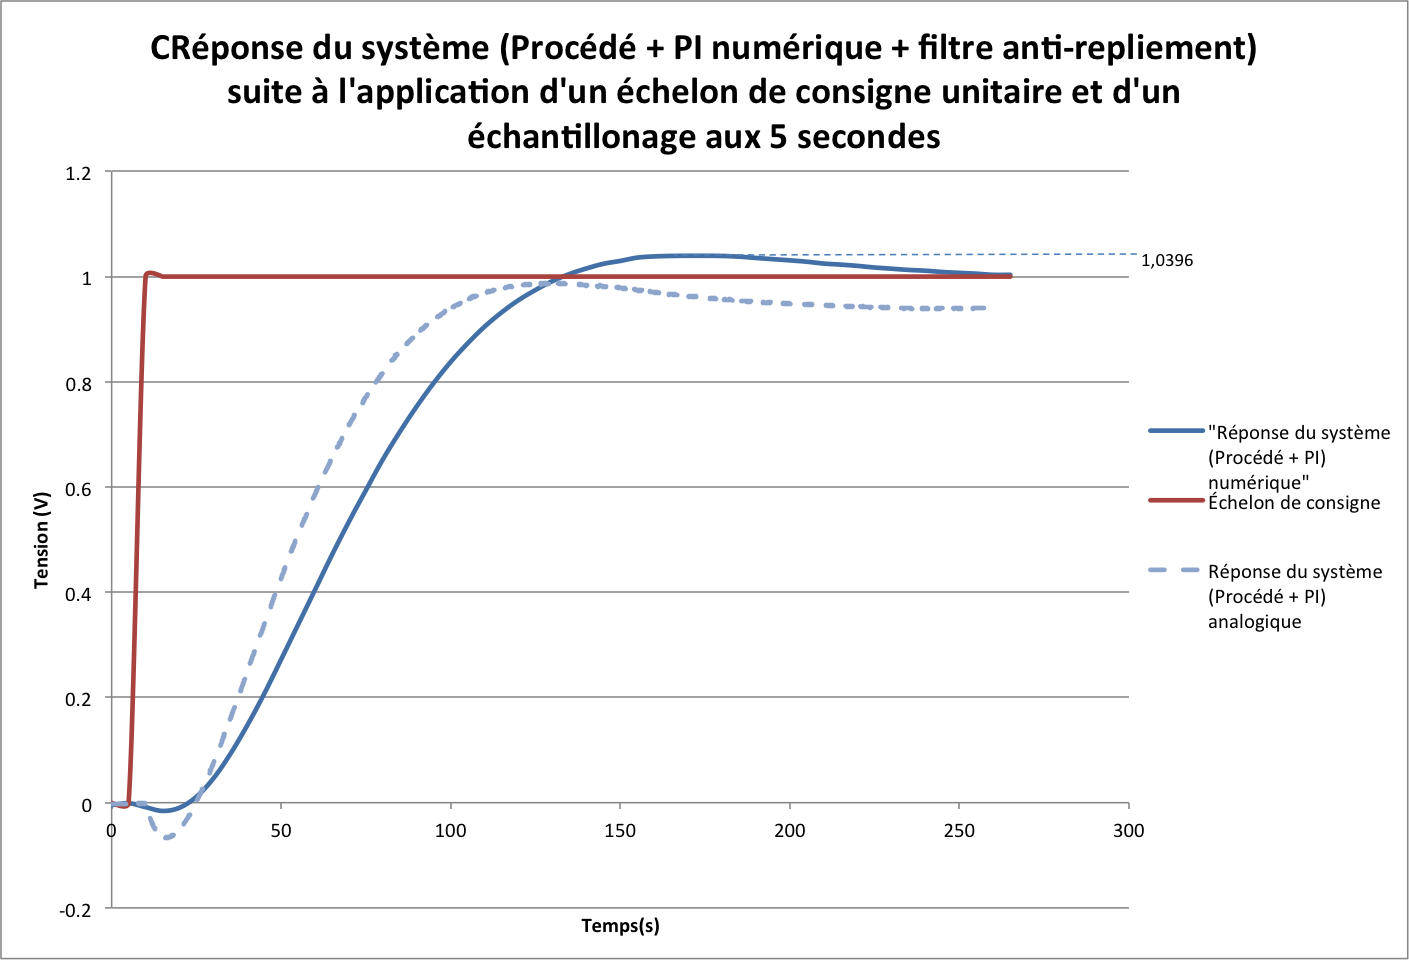
\includegraphics[scale=0.6]{fig_essai_numerique.png}
\caption{Essai de validation des performances de l'asservissement numérique du procédé}
\label{fig6}
\end{figure}
